% 图 B.3 点电荷电场：正电荷场线发散、负电荷场线汇聚（补全上半幅）
\documentclass[tikz,border=5pt]{standalone}
\usetikzlibrary{arrows.meta}
\usepackage{amsmath}
\usepackage{bm}
\usepackage{fontspec}
\setmainfont{Times New Roman}
\begin{document}
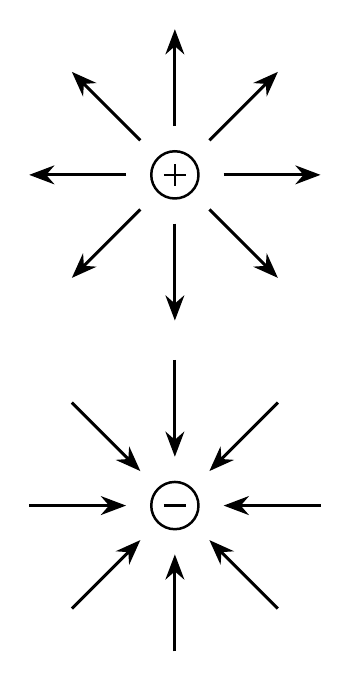
\begin{tikzpicture}[line width=0.8pt,>=Stealth]
\tikzset{fld/.style={line width=1.1pt,-{Stealth[length=3.2mm,width=2.4mm]}}}
% ---------- top: positive charge, field lines diverge ----------
\begin{scope}[shift={(0,2.1)}]
  \foreach \a in {0,45,...,315}{ \draw[fld] (\a:0.62) -- (\a:1.85); }
  \draw[line width=0.9pt,fill=white] (0,0) circle (0.30);
  \draw[line width=0.9pt] (-0.14,0) -- (0.14,0);
  \draw[line width=0.9pt] (0,-0.14) -- (0,0.14);
\end{scope}
% ---------- bottom: negative charge, field lines converge ----------
\begin{scope}[shift={(0,-2.1)}]
  \foreach \a in {0,45,...,315}{ \draw[fld] (\a:1.85) -- (\a:0.62); }
  \draw[line width=0.9pt,fill=white] (0,0) circle (0.30);
  \draw[line width=0.9pt] (-0.14,0) -- (0.14,0);
\end{scope}
\end{tikzpicture}
\end{document}
